% Technical Report -- Track 2, AI for MEMS (max 3 pages)
% Build:  pdflatex 02_technical_report.tex  (twice)
% Requires: IEEEtran.cls, booktabs, graphicx, amsmath
\documentclass[conference,10pt]{IEEEtran}
\usepackage{booktabs,graphicx,amsmath,amssymb,balance}
\graphicspath{{../figures/}}

\title{Differentiable MEMS Pull-In:\\Inverse Design Through a Bifurcation}
\author{\IEEEauthorblockN{Tushar Dudeja}}

\begin{document}
\maketitle

\begin{abstract}
Electrostatic pull-in is a saddle-node bifurcation that limits MEMS actuator
travel and destroys devices when crossed. We present a differentiable solver
that targets the bifurcation \emph{directly}, via the extended fold system, and
therefore yields exact gradients of the pull-in voltage with respect to device
geometry. This enables three data-free AI capabilities: gradient-based inverse
design, an amortized design network trained end-to-end through the physics with
no stored simulations, and a reinforcement-learning policy that infers each
device's unmeasurable fabrication ceiling. The solver is validated against eight
independent sources spanning 1967--2025, reproducing a published \emph{reversal}
of the optimal gap exponent between cantilever and fixed--fixed geometries. The
amortized network emits a specification-satisfying geometry in $0.04$\,ms,
matching converged optimization, and the control policy recovers
$80.4\pm4.9\%$ of travel lost to conservatism with zero devices destroyed.
\end{abstract}

\section{Method}

\subsection{Governing equations}
A beam of plate modulus $\tilde{E}$ and thickness $t$ over a shaped electrode
gap $d(x)$ obeys, in nondimensional form ($x=l\xi$, $y=d_0Y$, $G=D-Y$),
\begin{equation}
Y'''' - N_t\,Y'' \;=\; \Lambda\,\frac{1+\alpha G}{G^{2}},
\label{eq:beam}
\end{equation}
with $\Lambda = 6\varepsilon_0V^2l^4/(\tilde{E}t^3d_0^3)$ the normalized load,
$N_t$ residual-stress tension and $\alpha$ a fringing correction. Discretized
by fourth-order finite differences, \eqref{eq:beam} gives a residual
$R(Y,\Lambda)$.

\subsection{Differentiating through the fold}
Pull-in is not a maximum of a smooth function but a \emph{turning point}: the
tangent stiffness $J=\partial R/\partial Y$ becomes singular. We therefore solve
the extended system of Keller and Seydel,
\begin{equation}
R(Y,\Lambda)=0,\qquad J(Y,\Lambda)\,v=0,\qquad v^{\!\top}v-1=0,
\label{eq:fold}
\end{equation}
for $(Y,\Lambda,v)$ in one Newton solve, warm-started from a coarse
displacement-controlled sweep. Gradients follow from the implicit function
theorem, so $\partial \Lambda_{\rm PI}/\partial d(x)$ is exact rather than a
finite-difference or surrogate estimate. Fig.~\ref{fig:fold}(a) shows the fold;
Fig.~\ref{fig:fold}(b) the deflection mode at that point.

Globalization matters: the solver uses an Armijo line search with a
fraction-to-the-boundary rule and row equilibration in the
displacement-controlled stage. Without the latter, an $O(1)$ constraint row
against $O(10^6)$ beam rows prevented convergence on shaped profiles.

\begin{figure}[t]
\centering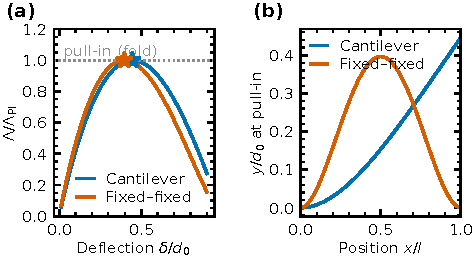
\includegraphics[width=\columnwidth]{Fig3_fold_structure.pdf}
\caption{(a) Equilibrium branch: the load maximum \emph{is} pull-in, the
saddle-node our solver targets. (b) Deflection profile at that point.}
\label{fig:fold}
\end{figure}

\section{Validation}

% Auto-generated by sim/make_tables.py -- do not edit by hand.
% Requires: \usepackage{booktabs}

\begin{table}[t]
\caption{Solver validation against independent published sources.
Errors are relative unless noted. ``mech.'' denotes the predicted
instability mechanism.}
\label{tab:validation}
\centering\footnotesize
\setlength{\tabcolsep}{3pt}
\begin{tabular}{@{}llrrr@{}}
\toprule
Source & Quantity & Ours & Published & Error \\
\midrule
Flores; Gomez \textit{et al.} & $\lambda^*$ (lumped)      & 0.148150 & 0.148148 & 0.001\% \\
Standard $\Lambda_{\rm PI}$   & cantilever                & 1.6799   & 1.6790   & 0.05\%  \\
Standard $\Lambda_{\rm PI}$   & fixed--fixed              & 69.935   & 71.167   & 1.73\%  \\
Analytic $c^3$ law            & $\sum \partial\Lambda/\partial D$ & 5.0398 & 5.0398 & 0.00\% \\
Seeger \& Boser, Tab.~I       & tip-in, design \#1        & 19.0\%   & 19\%     & --- \\
Seeger \& Boser, Tab.~I       & tip-in, design \#3        & 85.1\%   & 85\%     & --- \\
Seeger \& Boser, Tab.~III     & mech., 3 designs          & 3/3      & 3/3      & --- \\
Nazemi \textit{et al.} 2025   & $V_{\rm PI}$ reduction    & 13.2\%   & 16.0\%   & 2.8\,pp \\
M-TEST (\emph{measured})      & $V_{\rm PI}$, 500\,\textmu m FB & 11.70\,V & 11.1$\pm$0.1\,V & +5.4\% \\
\bottomrule
\end{tabular}
\end{table}


\begin{table}[t]
\caption{Inverse design versus the published hand-tuned study
(Haluzan \textit{et al.}), both boundary conditions, all designs re-fitted to
2\,\textmu m stable travel. The optimal exponent \emph{reverses} between the
two cases, which our solver reproduces.}
\label{tab:inverse}
\centering\footnotesize
\setlength{\tabcolsep}{3pt}
\begin{tabular}{@{}lrrrr@{}}
\toprule
& \multicolumn{2}{c}{Cantilever} & \multicolumn{2}{c}{Fixed--fixed} \\
\cmidrule(lr){2-3}\cmidrule(lr){4-5}
Design & Ours & Paper & Ours & Paper \\
\midrule
Uniform gap            & 22.86 & 23.66 & 175.83 & 178.26 \\
Linear ($n{=}1$)       & 14.31 & 14.86 & 123.01 & 125.48 \\
Best published family  & 13.61 & 14.14 & 121.79 & 123.94 \\
Free-form (ours)       & \textbf{13.60} & --- & \textbf{120.03} & --- \\
\midrule
Optimal exponent $n^*$ & 1.29 & 4/3 & 1.00 & 1.00 \\
Gain over best family  & 0.14\% & --- & 1.45\% & --- \\
\bottomrule
\end{tabular}
\end{table}


\begin{table}[t]
\caption{Design methods on the same task (cantilever, 2\,\textmu m travel).
Surrogate and direct rows share an equal budget of 400 true fold solves;
all designs are scored at exactly 2\,\textmu m travel by the exact solver.}
\label{tab:methods}
\centering\footnotesize
\setlength{\tabcolsep}{3pt}
\begin{tabular}{@{}lrrr@{}}
\toprule
Method & $V_{\rm PI}$ [V] & Train. samples & Design time \\
\midrule
MLP surrogate + active learning & 17.203 & 400 & 71\,s \\
FNO surrogate + active learning & 14.245 & 400 & 594\,s \\
Direct differentiable (400)     & 13.783 & 0   & 15\,s \\
Direct, converged (4 restarts)  & 13.665 & 0   & 170\,s \\
Amortized network               & 13.636 & \textbf{0} & \textbf{0.04\,ms} \\
Network $+$ 100 steps           & \textbf{13.599} & 0 & 17\,s \\
\midrule
\multicolumn{4}{@{}l@{}}{\footnotesize Hand-tuned published design: 14.14\,V.
Network training: 1577\,s, 6000 live solves, 0 stored.} \\
\bottomrule
\end{tabular}
\end{table}



Table~\ref{tab:validation} and Fig.~\ref{fig:valid} summarize agreement with
eight independent sources. Two results are load-bearing. First, the exact
gradient reproduces the analytic $c^3$ scaling law to $0.00\%$, confirming that
differentiation through \eqref{eq:fold} is correct and not merely plausible.
Second, the \emph{optimal gap exponent reverses} between geometries
(Fig.~\ref{fig:design}(b),(c)): $n^*\!=\!1.29$ for cantilevers against a
published $4/3$, and $n^*\!=\!1.00$ for fixed--fixed beams, matching the
published monotone trend. Opposite trends in two geometries are not obtainable
by fitting.

\begin{figure}[t]
\centering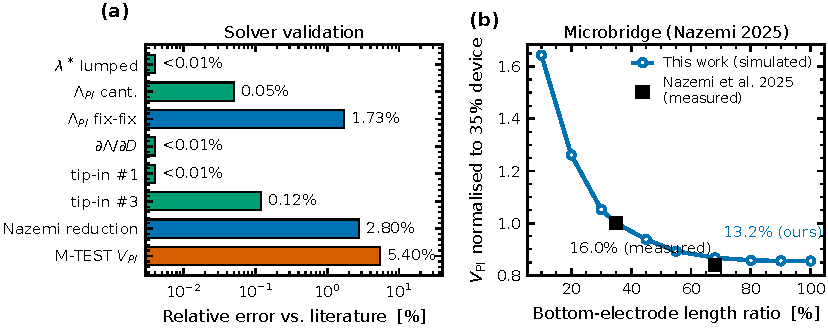
\includegraphics[width=\columnwidth]{Fig4_validation.pdf}
\caption{(a) Relative error against every source checked. (b) Normalized
pull-in versus electrode-length ratio for a 2025 measured microbridge; absolute
voltages are offset by anchor compliance (Sec.~\ref{sec:limits}), so the
comparison is normalized as in the source.}
\label{fig:valid}
\end{figure}

\section{Inverse design}

Minimizing $V_{\rm PI}$ subject to a fixed stable-travel specification is
solved by gradient descent on a free-form gap profile, with the scale set by a
differentiable constraint layer so every iterate is feasible. Starting from a
\emph{uniform} gap and given no knowledge of the published design family, the
optimizer rediscovers the published profile (Fig.~\ref{fig:design}(a)) and
descends $22.9\rightarrow13.9$\,V unaided. Table~\ref{tab:inverse} reports both
boundary conditions.

This also settles an open question: Haluzan \emph{et al.} conjectured that gains
beyond simple shapes ``are believed to be minimal.'' Free-form optimization over
the entire profile yields $0.14\%$ (cantilever) and $1.45\%$ (fixed--fixed).

\begin{figure*}[t]
\centering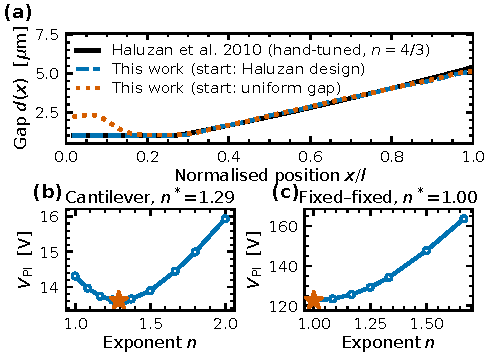
\includegraphics[width=\textwidth]{Fig1_solver_and_inverse_design.pdf}
\caption{(a) The optimizer rediscovers the published hand-tuned profile from a
uniform-gap start. (b),(c) The optimal exponent \emph{reverses} between
geometries; both are reproduced.}
\label{fig:design}
\end{figure*}

\section{AI methods}

\subsection{Amortized design without a dataset}
A network maps a specification (required travel) to a geometry and is trained
by backpropagating through \eqref{eq:fold}. There is no training set: every
gradient comes from a live solve. A soft penalty on the constraint proved
biased ($\sim$5\% specification error), because reducing travel also reduces
$V_{\rm PI}$; replacing it with a differentiable \emph{enforcement layer}
(OptNet/HardNet-style, implicit-function backprop) reduced the error to
$0.75\%$ (Fig.~\ref{fig:amort}). Inference costs $0.04$\,ms against
$\sim$30\,s for optimization, and the one-time training amortizes after
$\approx$53 designs.

\subsection{Comparison with surrogate modeling}
Standard practice fits a surrogate to $\sim$10$^4$ simulations. At an
\emph{equal budget} of 400 solves, an MLP surrogate reaches 17.20\,V and a
Fourier Neural Operator 14.25\,V, against 13.78\,V for direct differentiation
(Table~\ref{tab:methods}). The FNO is competitive; our advantage is that it
requires no training data, no architecture search and $40\times$ less
wall-clock, not superior accuracy.

\subsection{RL for unmeasurable fabrication variance}
The tip-in ceiling $r_{\rm ti}=1/(1+k_xL_c^2/6k_\theta)$ varies per device and
is not measurable at test time, so fixed-gain control must target the
worst case, forfeiting $19\%$ of travel. A policy observing only the device's
own tilt response recovers $80.4\pm4.9\%$ of that range with
$0.0\pm0.0\%$ devices destroyed over 1{,}536 episodes. That it truly
\emph{adapts} rather than being uniformly less conservative is shown by the
correlation between achieved travel and each device's ceiling:
$\rho=+0.96$ versus $-0.03$ for fixed gain (Fig.~\ref{fig:ai}(a)).

\begin{figure*}[t]
\centering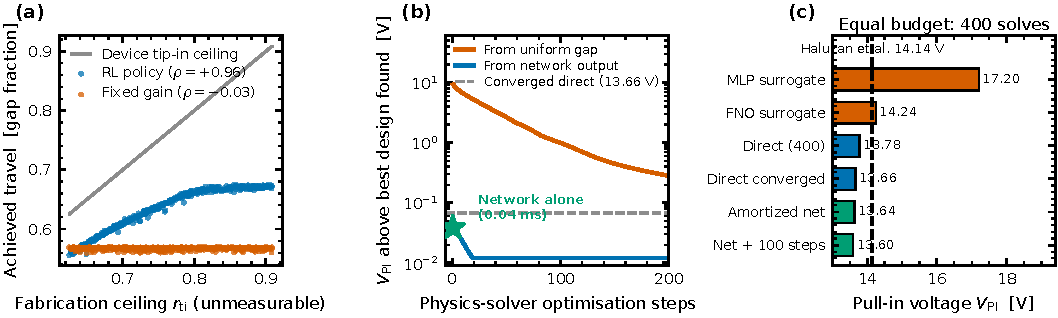
\includegraphics[width=\textwidth]{Fig2_ai_design_and_control.pdf}
\caption{(a) The policy tracks each device's unmeasurable ceiling. (b) A
learned initialization reaches better designs in 5 steps than a cold start
does in 500. (c) All methods at an equal 400-solve budget.}
\label{fig:ai}
\end{figure*}

\begin{figure}[t]
\centering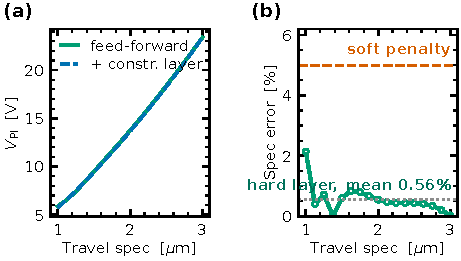
\includegraphics[width=\columnwidth]{Fig5_amortized_sweep.pdf}
\caption{Amortized network across the whole specification range. (a) Output
quality. (b) The hard-constraint layer cuts specification error from
$\sim$5\% to $0.75\%$.}
\label{fig:amort}
\end{figure}

\section{Limitations}\label{sec:limits}

Absolute voltages carry a systematic offset: $+5.4\%$ against the M-TEST
measurement, and $\sim$$+85\%$ for the 2025 microbridge, where matching would
require an effective length of $162\,\mu$m against a drawn $120\,\mu$m. The
evidence points to anchor compliance, absent from our ideal-clamp 1D model;
relative and trend predictions agree within 2.8\,pp. The static solver requires
float64 (fp32 does not converge, $|R|=2.0$ versus $10^{-8}$) and is therefore
CPU-bound on consumer GPUs. The amortized network \emph{matches} rather than
beats converged optimization (13.636 vs 13.665\,V, within the 0.28\% spread
across restarts). Finally, fixed--fixed profiles with $n\gtrsim1.8$ are
infeasible rather than merely costly: travel saturates below specification at
any scale, and they are excluded rather than plotted.

\balance
\begin{thebibliography}{9}\footnotesize
\bibitem{osterberg} P.~M. Osterberg and S.~D. Senturia, ``M-TEST,''
\emph{J. Microelectromech. Syst.}, vol.~6, pp.~107--118, 1997.
\bibitem{haluzan} D.~Haluzan \emph{et al.}, ``Reducing pull-in voltage by
adjusting gap shape,'' \emph{Micromachines}, vol.~1, pp.~68--81, 2010.
\bibitem{seeger} J.~I. Seeger and B.~E. Boser, ``Charge control of
parallel-plate electrostatic actuators and the tip-in instability,''
\emph{J. Microelectromech. Syst.}, vol.~12, pp.~656--671, 2003.
\bibitem{nazemi} H.~Nazemi \emph{et al.}, ``Microbridge resonators for reduced
pull-in voltage,'' \emph{J. Sens. Sens. Syst.}, vol.~14, pp.~219--225, 2025.
\bibitem{keller} H.~B. Keller, ``Numerical solution of bifurcation and
nonlinear eigenvalue problems,'' 1977.
\bibitem{nathanson} H.~C. Nathanson \emph{et al.}, ``The resonant gate
transistor,'' \emph{IEEE Trans. Electron Devices}, vol.~ED-14, 1967.
\bibitem{zhang} L.~Zhang \emph{et al.}, ``Machine learning-driven metastructure
design,'' \emph{Microsyst.\ Nanoeng.}, vol.~11, 214, 2025.
\bibitem{blau} T.~Blau \emph{et al.}, ``Optimizing sequential experimental
design with deep RL,'' \emph{ICML}, 2022.
\end{thebibliography}

\end{document}
